% ADS Project 2 -- Dijkstra with four priority queues
% This report is self-contained and uses data recorded in the repository.

\documentclass[12pt,a4paper]{report}
\usepackage[utf8]{inputenc}
\usepackage[T1]{fontenc}
\usepackage{geometry}
\usepackage{amsmath,amssymb}
\usepackage{graphicx}
\usepackage{booktabs}
\usepackage{float}
\usepackage{caption}
\usepackage{titlesec}
\usepackage{enumitem}
\usepackage{xcolor}
\usepackage{algorithm}
\usepackage{algorithmicx}
\usepackage{algpseudocode}
\usepackage{indentfirst}
\usepackage{multirow}
\usepackage{hyperref}
\usepackage{pgfplots}

\geometry{left=2.5cm,right=2.5cm,top=2.5cm,bottom=2.5cm}
\setlength{\parindent}{2em}
\setlength{\parskip}{1pt}

\titleformat{\chapter}
  {\normalfont\LARGE\bfseries}
  {\chaptername\ \thechapter.\quad}
  {0pt}
  {}
\titlespacing*{\chapter}{0pt}{0pt}{20pt}

\titleformat{\section}
  {\normalfont\large\bfseries}
  {\thesection}
  {1em}
  {}
\titlespacing*{\section}{0pt}{12pt}{6pt}

\titleformat{\subsection}
  {\normalfont\normalsize\bfseries}
  {\thesubsection}
  {1em}
  {}
\titlespacing*{\subsection}{0pt}{10pt}{4pt}

\setlist[itemize]{left=0pt,topsep=4pt,partopsep=0pt,itemsep=2pt}
\setlist[enumerate]{left=0pt,topsep=4pt,partopsep=0pt,itemsep=2pt}

\hypersetup{colorlinks=true,linkcolor=blue,urlcolor=blue,citecolor=blue}
\pgfplotsset{compat=1.18}
\newcommand{\code}[1]{\texttt{\detokenize{#1}}}

\begin{document}

% ------------------------------- title page -------------------------------
\begin{center}
  {\Huge\bfseries Performance Comparison of\\[0.35cm]
   Four Priority Queues for Dijkstra's Algorithm\par}
  \vspace{1.5cm}
  \Large Course: Data Structures and Algorithms\\[0.35cm]
  \Large Project: Shortest Path Algorithm with Heaps\\[0.35cm]
  \Large Implementation: C (C11 / C++17-compatible C style)\\[0.35cm]
  \Large Completion Date: October 25, 2026\\[1.2cm]
  \Large You Longbin \quad 3250106392\\
  \vspace{0.4cm}
  \Large Huang Yirui \quad 3250104426\\
  \vspace{0.4cm}
  \Large Chen Zhikun \quad 3250100883\\
  \vspace{1.5cm}
  \Large Generated with \LaTeX
\end{center}

\newpage
\tableofcontents
\newpage

% ============================== Chapter 1 ================================
\chapter{Introduction}

\section{Description}
The single-source shortest-path problem asks for the minimum path cost from a
source vertex to every other vertex in a weighted graph. When all edge weights
are non-negative, Dijkstra's algorithm solves this problem by repeatedly
selecting the unsettled vertex with the smallest tentative distance and
relaxing its outgoing edges. A min-priority queue supports this selection and
the key updates caused by successful relaxations.

The project asks us to implement Dijkstra's algorithm with multiple heap
structures and determine which implementation performs best on USA road
networks. The evaluation uses three DIMACS graphs, NY, COL, and FLA, with 1,000
distinct source--target queries per graph. After one complete warm-up,
each batch is measured three times and summarized by its median and
observed range. The implementation compares four
min-priority queues: binary, ternary, Fibonacci, and binomial heaps. Including
four structures exceeds the assignment's two-structure minimum and includes
the required Fibonacci heap.

The measured task is a point-to-point query rather than a complete single-source
run. Each query terminates as soon as the target is extracted as the current
minimum. This early termination makes the tested workload smaller than a full
traversal and makes the operation mix, query distribution, and queue
implementation important to the result.

\section{Overview of the Implementation}
The program is organized around four shared components.

\begin{enumerate}
  \item \textbf{Graph loading.} The DIMACS road network is parsed into a
        compressed sparse row (CSR) representation. An offset array identifies
        each vertex's outgoing-arc range, while one contiguous edge array stores
        destinations and non-negative weights.
  \item \textbf{Priority queues.} Each heap implements insertion,
        extract-min, decrease-key, and clearing after a query. The two array
        heaps use a vertex-position array; the linked heaps use their tree and
        root-list structures.
  \item \textbf{Dijkstra query runner.} A common search procedure is run with
        each heap. It stops at the target, records high-level operation counts,
        and uses the same deterministic comparison order, $(distance, vertex
        ID)$, for every implementation.
  \item \textbf{Benchmark and output.} A deterministic generator creates the
        query pairs. The program records runtimes, returned distances, and
        Dijkstra-level work in CSV files. A separate count-only build records
        internal heap operations without adding those counter updates to the
        timed build.
\end{enumerate}

Chapter 2 specifies the common search and summarizes the four heaps. Chapter 3
presents the input graphs, evaluation procedure, correctness cross-check,
runtime table, and plot. Chapter 4 focuses on the measured causes of the
performance differences and states the limits of the evidence. The appendix
points to the complete source without duplicating implementation code.

% ============================== Chapter 2 ================================
\chapter{Algorithm Specification}

\section{Graph and Priority-Queue Data Structures}
Let $G=(V,E)$ be a directed graph with non-negative edge weights. The graph is
stored in CSR form: \code{offset[u]} through \code{offset[u+1]-1} index the
outgoing arcs of vertex $u$. The edge array stores the destination and weight
for each arc. This representation requires $O(V+E)$ memory and avoids the
$O(V^2)$ space of an adjacency matrix.

Each queue item is ordered lexicographically by its key and vertex ID. This
gives deterministic tie-breaking when two tentative distances are equal. The
queue API is the same for all four heaps: insert a vertex, extract the
minimum-key item, decrease a queued vertex's key, check whether the queue is
empty, and clear the remaining items after a query.

\begin{table}[H]
  \centering
  \caption{Priority-queue representations and operation costs}
  \label{tab:heap-operations}
  \small
  \begin{tabular}{p{1.7cm}p{4.4cm}p{2.0cm}p{2.3cm}p{2.3cm}}
    \toprule
    Heap & Representation & Insert & Extract-min & Decrease-key \\
    \midrule
    Binary & Array; vertex-position map & $O(\log q)$ & $O(\log q)$ & $O(\log q)$ \\
    Ternary & Array; three-way branching; position map & $O(\log q)$ & $O(\log q)$ & $O(\log q)$ \\
    Fibonacci & Circular root/child lists; consolidation and cuts & $O(1)$ amort. & $O(\log q)$ amort. & $O(1)$ amort. \\
    Binomial & Degree-ordered tree roots & $O(\log q)$ & $O(\log q)$ & $O(\log q)$ \\
    \bottomrule
  \end{tabular}
  \vspace{2pt}

  \footnotesize $q$ denotes the current number of items in the priority queue.
\end{table}

The two array heaps differ only in branching factor. The Fibonacci heap uses
root and child lists with consolidation after extract-min; the binomial heap
uses degree-ordered trees. These structural differences are relevant to the
performance analysis in Chapter 4; implementation-level code is in
\code{src/1.c}.

\section{Dijkstra Query Algorithm}
\noindent\textbf{Input}: Directed graph $G$ with non-negative edge weights,
source $s$, target $t$, and an empty min-priority queue $Q$\\
\textbf{Output}: The shortest-path distance from $s$ to $t$, or $\infty$ if
no path exists

\begin{algorithm}[H]
  \begin{algorithmic}[1]
    \ForAll{$v \in V$}
      \State $dist[v] \gets \infty$
      \State $state[v] \gets \text{UNSEEN}$
    \EndFor
    \State $dist[s] \gets 0$
    \State \Call{Insert}{$Q,s,0$}
    \State $state[s] \gets \text{IN\_QUEUE}$
    \While{$Q$ is not empty}
      \State $(u,d) \gets$ \Call{ExtractMin}{$Q$}
      \State $state[u] \gets \text{SETTLED}$
      \If{$u=t$}
        \State \Return $d$
      \EndIf
      \ForAll{arcs $(u,v,w)$ leaving $u$}
        \If{$state[v] \neq \text{SETTLED}$ and $d+w < dist[v]$}
          \State $dist[v] \gets d+w$
          \If{$state[v] = \text{UNSEEN}$}
            \State \Call{Insert}{$Q,v,dist[v]$}
            \State $state[v] \gets \text{IN\_QUEUE}$
          \Else
            \State \Call{DecreaseKey}{$Q,v,dist[v]$}
          \EndIf
        \EndIf
      \EndFor
    \EndWhile
    \State \Return $\infty$
  \end{algorithmic}
  \caption{Point-to-point Dijkstra query with early termination}
  \label{alg:dijkstra-query}
\end{algorithm}

The search is correct because all edge weights are non-negative. When a
vertex is extracted with the smallest tentative distance, no path through an
unsettled vertex can later produce a shorter distance to it; its distance is
therefore final. The target's distance is final when it is extracted, so the
query may stop at that point. All four implementations receive the same
source--target pairs and use the same tie-breaking rule.

The pseudocode shows logical initialization for clarity. The implementation
allocates the workspace once and resets only vertices touched by each query;
remaining queue entries are cleared before the next query.

\section{Theoretical Complexity}
For a complete single-source run, each vertex is extracted once and each edge
may cause a successful relaxation. With $q\leq V$, the standard bounds are
shown in Table~\ref{tab:complexity}. The point-to-point benchmark can stop
earlier; its actual work depends on the portion of the graph settled before
the target is extracted.

\begin{table}[H]
  \centering
  \caption{Complete single-source Dijkstra bounds}
  \label{tab:complexity}
  \begin{tabular}{lcc}
    \toprule
    Priority queue & Time & Additional queue space \\
    \midrule
    Binary heap & $O((V+E)\log V)$ & $O(V)$ \\
    Ternary heap & $O((V+E)\log V)$ & $O(V)$ \\
    Fibonacci heap & $O(E+V\log V)$ amortized & $O(V)$ \\
    Binomial heap & $O((V+E)\log V)$ & $O(V)$ \\
    \bottomrule
  \end{tabular}
\end{table}

The Fibonacci bound follows from amortized $O(1)$ insertion and decrease-key
and amortized $O(\log V)$ extract-min. The other three structures use
$O(\log V)$ for each of these operations. These asymptotic bounds do not by
themselves predict the fastest implementation: operation frequencies,
constant costs, memory layout, and the early-stop query workload also affect
runtime.

% ============================== Chapter 3 ================================
\chapter{Testing Results}

\section{Test Cases and Input Data}
The evaluation uses three DIMACS USA road networks. Each graph contains
directed arcs with integer, non-negative distance weights. A deterministic
xorshift generator creates 1,000 distinct ordered source--target pairs per
graph; each pair has different source and target vertices. The same query list
is passed to all four heaps.

\begin{table}[H]
  \centering
  \caption{Road-network input sizes and query counts}
  \label{tab:datasets}
  \begin{tabular}{lrrrr}
    \toprule
    Dataset & Vertices $V$ & Directed arcs $E$ & $E/V$ & Queries \\
    \midrule
    NY  & 264,346 & 733,846   & 2.78 & 1,000 \\
    COL & 435,666 & 1,057,066 & 2.43 & 1,000 \\
    FLA & 1,070,376 & 2,712,798 & 2.53 & 1,000 \\
    \bottomrule
  \end{tabular}
\end{table}

The official dataset page and download links are listed below, as required by
the assignment. The report does not attach the raw road-network files.

\begin{itemize}
  \item \href{https://www.diag.uniroma1.it/challenge9/download.shtml}{DIMACS Challenge 9 data page}
  \item \href{https://www.diag.uniroma1.it/challenge9/data/USA-road-d/USA-road-d.NY.gr.gz}{NY graph download (USA-road-d.NY.gr.gz)}
  \item \href{https://www.diag.uniroma1.it/challenge9/data/USA-road-d/USA-road-d.COL.gr.gz}{COL graph download (USA-road-d.COL.gr.gz)}
  \item \href{https://www.diag.uniroma1.it/challenge9/data/USA-road-d/USA-road-d.FLA.gr.gz}{FLA graph download (USA-road-d.FLA.gr.gz)}
\end{itemize}

The local graph files were reconstructed from publicly available FROM, TO,
and W edge arrays after the official DIMACS host could not be reached during
data preparation. Their vertex and arc counts match the published counts,
but the local files have not been checked arc by arc against the official
downloads. The provenance is documented in \path{data/dimacs/README.md}.

\section{Measurement Method}
The experiment was reproduced on October 25, 2026, on an Apple M1 Max
with 32 GiB of memory and 10 CPU cores, running macOS 26.6.2.
The unchanged C source was compiled with Apple Clang 21.0.0 in C11 mode
using \code{-O2}, \code{-Wall}, and \code{-Wextra}. Execution is single-threaded.

One complete warm-up was followed by three complete measured program runs.
Each run used the same 1,000 distinct source--target pairs per network,
giving three observations per heap and graph, or 36,000 timed query
executions overall. The reported times are medians across the three
1,000-query batches. Repetition measures run-to-run variation on a fixed
workload; there are still 1,000 distinct pairs per graph.

The program uses \code{clock()} to measure CPU time around each batch.
Graph loading, query generation, and workspace/heap allocation are excluded;
per-query heap and state cleanup is included. Warm-up times are excluded.
The starting heap rotates by dataset; each dataset keeps the same heap order
across repetitions. Queries, answers, and high-level operation counts were
checked for exact agreement across the warm-up and all three measured runs.
Machine details, compiler flags, and input/source hashes are recorded in
\path{results/benchmark_environment.json}.

Detailed heap counters are disabled in the timing build. The existing
internal-counter CSV is retained from the earlier implementation's separate
counting pass. It is used only as legacy structural-work evidence in
Chapter 4, not as a time breakdown of this local experiment.

\section{Correctness Cross-Check}
On every road network and in every measured repetition, all four heaps
returned identical distances for all 1,000 query pairs. The query sequence,
answers, and Dijkstra-level work were identical across repetitions.

A Python implementation of Floyd--Warshall provided an independent
reference on three synthetic 40-vertex graphs. These fixtures
cover connected and disconnected graphs, zero-weight and parallel edges,
isolated vertices, and path distances beyond 32-bit integer range.
All 12,000 heap answers for 3,000 query pairs matched the oracle, including
1,122 unreachable pairs and 330 distances above $2^{31}-1$.
These synthetic tests are separate from the road-network timings.
The check and its record are available in
\path{scripts/check_shortest_paths.py} and \path{results/reference_checks.json}.
Together with the Chapter 2 argument, they provide independent evidence for
the tested cases.

\section{Run-Time Results}
Table~\ref{tab:runtime} reports median total CPU seconds for 1,000-query
batches over three repetitions. Since each batch contains 1,000 queries,
its total seconds are numerically equal to its average milliseconds per
query. Table~\ref{tab:runtime-ranges} gives the observed minimum and maximum.
The raw observations, means, and sample standard deviations are stored in
the repetition and statistics CSV files.

\begin{table}[H]
  \centering
  \small
  \caption{Median total CPU time for 1,000 queries, three repetitions (seconds)}
  \label{tab:runtime}
  \begin{tabular}{lrrrrc}
    \toprule
    Dataset & Binary & Ternary & Fibonacci & Binomial & Matches per run \\
    \midrule
    NY & 12.744 & 11.608 & 24.264 & 21.850 & 1,000/1,000 \\
    COL & 20.584 & 18.823 & 37.767 & 33.708 & 1,000/1,000 \\
    FLA & 51.513 & 47.112 & 96.150 & 85.851 & 1,000/1,000 \\
    \bottomrule
  \end{tabular}
\end{table}
\begin{table}[H]
  \centering
  \small
  \caption{Observed minimum--maximum times across three repetitions (seconds)}
  \label{tab:runtime-ranges}
  \begin{tabular}{lrrrr}
    \toprule
    Dataset & Binary & Ternary & Fibonacci & Binomial \\
    \midrule
    NY & 12.688--12.767 & 11.569--11.647 & 24.263--24.267 & 21.822--21.904 \\
    COL & 20.482--20.662 & 18.787--18.950 & 37.621--37.968 & 33.631--33.759 \\
    FLA & 51.370--51.790 & 47.067--47.963 & 95.916--96.385 & 85.570--86.079 \\
    \bottomrule
  \end{tabular}
\end{table}

\begin{figure}[H]
  \centering
  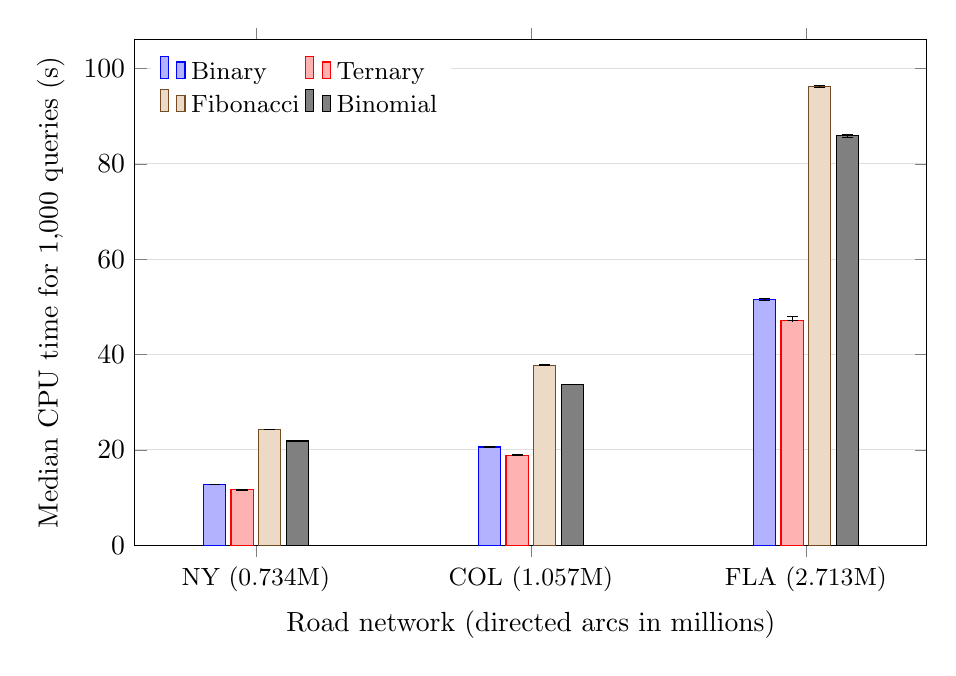
\begin{tikzpicture}
    \begin{axis}[
      ybar, bar width=8pt, width=0.96\linewidth, height=8cm, ymin=0,
      ylabel={Median CPU time for 1,000 queries (s)},
      xlabel={Road network (directed arcs in millions)},
      symbolic x coords={NY,COL,FLA}, xtick=data,
      xticklabels={NY (0.734M),COL (1.057M),FLA (2.713M)},
      x tick label style={font=\small}, ymajorgrids=true,
      grid style={gray!25}, enlarge x limits=0.22,
      legend style={at={(0.02,0.98)},anchor=north west,legend columns=2,
                    font=\small,draw=none,fill=white}, legend cell align=left
    ]
      \addplot+[error bars/.cd,y dir=both,y explicit,error bar style={black}] coordinates {(NY,12.744330) +=(0,0.022292) -=(0,0.056512) (COL,20.584066) +=(0,0.077713) -=(0,0.102173) (FLA,51.513346) +=(0,0.276741) -=(0,0.143749)};
      \addplot+[error bars/.cd,y dir=both,y explicit,error bar style={black}] coordinates {(NY,11.607607) +=(0,0.039331) -=(0,0.038411) (COL,18.822622) +=(0,0.127060) -=(0,0.036079) (FLA,47.111732) +=(0,0.851168) -=(0,0.044973)};
      \addplot+[error bars/.cd,y dir=both,y explicit,error bar style={black}] coordinates {(NY,24.264308) +=(0,0.002642) -=(0,0.001264) (COL,37.767477) +=(0,0.200273) -=(0,0.146622) (FLA,96.149886) +=(0,0.234888) -=(0,0.234069)};
      \addplot+[error bars/.cd,y dir=both,y explicit,error bar style={black}] coordinates {(NY,21.850092) +=(0,0.054236) -=(0,0.027823) (COL,33.708046) +=(0,0.051217) -=(0,0.076649) (FLA,85.850519) +=(0,0.228733) -=(0,0.280982)};

      \legend{Binary,Ternary,Fibonacci,Binomial}
    \end{axis}
  \end{tikzpicture}
  \caption{Median runtime versus graph size; whiskers show observed minimum
  and maximum across three repetitions.}
  \label{fig:runtime}
\end{figure}

The ternary heap was fastest in all three repetitions on each network.
The binary heap followed, then binomial and Fibonacci. These are observations
for this machine, compiler, and query set. The networks differ in structure
as well as size, so the plot does not isolate arc count as a cause of runtime.
Whiskers describe observed variation and are not confidence intervals.

\section{Dijkstra Work Performed}
The following counts are totals over the 1,000 queries on each dataset. All
four implementations perform the same high-level Dijkstra work on a given
graph, with identical counts in all three repetitions.

\begin{table}[H]
  \centering
  \caption{Shared Dijkstra-level operation counts over 1,000 queries}
  \label{tab:work}
  \small
  \begin{tabular}{lrrrr}
    \toprule
    Dataset & Scanned arcs & Extract-min & Insert & Successful decrease-key \\
    \midrule
    NY  & 385,059,749 & 135,502,866 & 135,947,390 & 19,297,309 \\
    COL & 541,176,229 & 220,809,144 & 221,168,701 & 16,421,882 \\
    FLA & 1,347,518,609 & 531,602,948 & 532,034,751 & 50,489,498 \\
    \bottomrule
  \end{tabular}
\end{table}

Extract-min outnumbers successful decrease-key by approximately 7.02, 13.45,
and 10.53 times on NY, COL, and FLA, respectively. Successful decrease-key
accounts for about 6.64\%, 3.58\%, and 4.53\% of the three queue operation
types combined. This workload fact is important when interpreting the
Fibonacci heap's amortized decrease-key advantage.

% ============================== Chapter 4 ================================
\chapter{Analysis and Comments}

\section{Time and Space Complexity Analysis}
For a complete single-source search, the graph representation takes
$O(V+E)$ space and each heap stores at most $V$ vertices. The queue-operation
bounds in Table~\ref{tab:heap-operations} yield the complete-search bounds in
Table~\ref{tab:complexity}. The measured point-to-point queries stop early, so
their actual number of settled vertices and scanned arcs may be substantially
smaller than $V$ and $E$ per query.

With $V_r$ settled vertices and $E_r$ scanned arcs in a particular query, the
binary, ternary, and binomial implementations perform
$O((V_r+E_r)\log V)$ queue work in the standard bound, since the active
frontier can contain vertices that have not yet been settled. The Fibonacci
implementation has amortized $O(E_r+V_r\log V)$ queue work. These are
asymptotic descriptions; the benchmark compares complete query batches and
does not isolate the cost of a single heap operation.

\section{Performance Comparison and Result Analysis}
All four implementations process the same queries and perform identical
Dijkstra-level work on each graph. The observed time gaps therefore arise
primarily from the heap operations and their implementation costs. The
operation counts below come from the independent legacy counter build; they
describe structural work, but are not a time decomposition of the optimized
timing build.

\subsection{Observed Runtime Ratios}
Table~\ref{tab:runtime-ratios} expresses the main timing results relative to
the binary heap. It makes the size and consistency of the gaps easier to see.

\begin{table}[H]
  \centering
  \small
  \caption{Median runtime relative to the binary heap in the local experiment}
  \label{tab:runtime-ratios}
  \begin{tabular}{lrrr}
    \toprule
    Dataset & Ternary / Binary & Fibonacci / Binary & Binomial / Binary \\
    \midrule
    NY & 0.911 & 1.904 & 1.714 \\
    COL & 0.914 & 1.835 & 1.638 \\
    FLA & 0.915 & 1.867 & 1.667 \\
    \bottomrule
  \end{tabular}
\end{table}


The ternary heap has the lowest median on all three networks. Fibonacci
takes 1.83--1.90 times the binary median,
while binomial takes 1.64--1.71 times the binary median.
For each graph, the observed binary and ternary ranges do not overlap.
Three repetitions document this local result but provide limited evidence
for rankings on other machines or query distributions.

The networks have only about 2.4--2.8 directed arcs per vertex.
With sparse graphs, substituting $E=O(V)$ into the full-search bounds makes
both array-heap and Fibonacci upper bounds $O(V\log V)$. This helps explain why
Fibonacci's general asymptotic bound need not yield a practical advantage here.

\subsection{Binary and Ternary: Height versus Child Checks}
The legacy counter pass recorded peak active queues of 1,002, 1,037, and 1,575 items on NY, COL, and
FLA. A binary heap at these sizes has roughly 10--11 levels. Both array heaps
therefore have short paths, contiguous storage, and direct vertex lookup via
the position array. A ternary heap shortens the downward path but examines up
to three children per level. This trade-off appears in the internal counters:

\begin{table}[H]
  \centering
  \caption{Ternary-heap internal counts relative to binary (legacy counter build)}
  \label{tab:array-counters}
  \small
  \begin{tabular}{lrrr}
    \toprule
    Dataset & Comparisons & Fewer downward iterations & Fewer array swaps \\
    \midrule
    NY  & $+0.55\%$ & $27.9\%$ & $32.2\%$ \\
    COL & $+0.93\%$ & $27.4\%$ & $32.4\%$ \\
    FLA & $+0.79\%$ & $27.6\%$ & $32.2\%$ \\
    \bottomrule
  \end{tabular}
\end{table}

The ternary heap consistently performs fewer downward iterations and swaps,
while making slightly more counted comparisons. Its observed median runtime
was lower than binary by 8.9\%, 8.6\%, 8.5\% on NY, COL,
and FLA, respectively. It was faster in all three paired repetitions
on each graph. Shorter paths and fewer swaps are consistent with this
result. Both structures use compact active arrays; cache locality and
branch behavior are plausible contributors, but hardware counters were
not collected.

\subsection{Why the Fibonacci Heap Is Slower Here}
The amortized $O(1)$ decrease-key operation is useful only when it forms a
substantial part of the workload. Here, successful decrease-key calls are
only 3.58--6.64\% of the three queue operation types, while extract-min is
performed 135.5--531.6 million times per dataset. Each Fibonacci extract-min
promotes children and consolidates roots, so this frequent operation incurs
linked-structure maintenance. Table~\ref{tab:fib-counters} summarizes the
legacy counters for the Fibonacci implementation.
In the following tables, B denotes one billion.

\begin{table}[H]
  \centering
  \caption{Fibonacci-heap structural work (legacy counter build)}
  \label{tab:fib-counters}
  \small
  \begin{tabular}{lrrrr}
    \toprule
    Dataset & Comparisons / Binary & Children / extract & Cuts / decrease & Tree links (B) \\
    \midrule
    NY  & 1.20$\times$ & 7.50 & 21.0\% & 1.02 \\
    COL & 1.20$\times$ & 7.10 & 23.1\% & 1.57 \\
    FLA & 1.20$\times$ & 7.45 & 19.8\% & 3.97 \\
    \bottomrule
  \end{tabular}
\end{table}

The legacy Fibonacci counter pass recorded about 20\% more key/item
comparisons than binary. Table~\ref{tab:fib-counters} shows about 7.1--7.5 child
promotions per extract-min and roughly one billion to four billion tree links
per dataset. Cuts happen on only about one fifth of successful decrease-key calls. Thus, this query
mix does not provide enough decrease-key work to compensate for repeated
extract-min consolidation and linked-list traversal.

Insertion is also amortized constant time in a Fibonacci heap and accounts
for roughly half of queue calls here. Lazy insertion defers consolidation to
extract-min, where the recorded child promotion and tree-link work occurs.
The current optimized degree table avoids a full unused-range scan, while
the structural costs of extraction remain.

\subsection{Why the Binomial Heap Is Slower Despite Fewer Comparisons}
The binomial heap records only about 70\% as many counted comparisons as the
binary heap, yet its local median takes 1.64--1.71 times as long. This illustrates why a
comparison counter is not a complete cost model. Degree comparisons
inside binomial root-list loops are excluded from that counter. Binomial operations also
merge degree-ordered root lists, link equal-degree trees, promote children,
and update parent/sibling pointers.

\begin{table}[H]
  \centering
  \caption{Binomial-heap structural work (legacy counter build)}
  \label{tab:binomial-counters}
  \small
  \begin{tabular}{lrrr}
    \toprule
    Dataset & Comparisons / Binary & Tree links (B) & Root-list steps (B) \\
    \midrule
    NY  & 0.70$\times$ & 1.04 & 4.09 \\
    COL & 0.70$\times$ & 1.61 & 6.37 \\
    FLA & 0.70$\times$ & 4.06 & 15.98 \\
    \bottomrule
  \end{tabular}
\end{table}

Its root-list step counter reaches 4.09 billion on NY and 15.98 billion on
FLA, consistent with substantial list traversal. The counter definitions
differ between Fibonacci and binomial heaps, so their root-list totals are
not directly comparable.

\section{Further Improvements and Measurement Limits}
\begin{enumerate}
  \item Three timed repetitions characterize observed variation for one
        deterministic query set. More repetitions and independently sampled
        pairs would support broader comparisons.
  \item Heap order rotates by dataset but stays fixed across repetitions.
        CPU frequency, thermal state, and background load were not locked.
        The min--max ranges are descriptive, not confidence intervals.
  \item Legacy internal counters describe an earlier implementation and
        provide structural context. They are not measurements of individual
        operation latency or a precise breakdown of the current CPU times.
  \item Only three sparse road networks were timed. Dense graphs and full
        single-source searches may have a different operation mix.
  \item Cache misses, branch behavior, and pointer-access costs were not
        profiled. Memory-locality explanations are interpretations of the
        structures and observations.
  \item The reconstructed graph files were count-checked but were not
        verified arc by arc against official files.
\end{enumerate}

\section{Summary}
In the three-run local experiment, ternary had the lowest median runtime on
NY, COL, and FLA, followed by binary, binomial, and Fibonacci. All measured
runs used identical queries and performed identical high-level graph work;
independent synthetic tests also matched a reference oracle.
The small active queues, low proportion of successful decrease-key calls,
and substantial linked-tree maintenance explain why asymptotic heap bounds
alone do not predict the measured ranking. The conclusions apply to this
source, machine, compiler, and query distribution.

\chapter*{References}
\addcontentsline{toc}{chapter}{References}
\begin{enumerate}[label={[\arabic*]}]
  \item Ye De-shi. \textit{Shortest Path Algorithm with Heaps}, Assignment
        8-1, Zhejiang University, course handout.
  \item DIMACS. \textit{9th DIMACS Implementation Challenge: Shortest Paths}.
        \href{https://www.diag.uniroma1.it/challenge9/download.shtml}{DIMACS download page}.
\end{enumerate}

\appendix
\chapter{Source Location}
The complete implementation is in \code{src/1.c}.
It contains DIMACS graph loading, all four priority queues, Dijkstra query
execution, deterministic query generation, runtime measurement, and CSV
output. Implementation details are summarized in Chapter 2; this report
focuses on their measured performance consequences.

Recorded files include:
\begin{itemize}
  \item Median timings: \path{results/benchmark_results.csv}.
  \item Raw repetitions: \path{results/benchmark_repetitions.csv}.
  \item Timing statistics: \path{results/benchmark_statistics.csv}.
  \item Queries: \path{results/benchmark_queries.csv}.
  \item Dijkstra work: \path{results/benchmark_operations.csv}.
  \item Legacy counters: \path{results/heap_internal_stats.csv}.
  \item Environment: \path{results/benchmark_environment.json}.
  \item Oracle checks: \path{results/reference_checks.json}.
  \item Run log: \path{results/benchmark_reproduction.log}.
\end{itemize}
The full timed experiment is reproduced with
\path{scripts/reproduce_benchmark.py}; the separate synthetic reference check
is in \path{scripts/check_shortest_paths.py}.

\end{document}
